\documentclass[12pt,letterpaper]{article}
% Essential packages
\usepackage[utf8]{inputenc}
\usepackage[margin=1in]{geometry}
\usepackage{graphicx}
\usepackage[x11names,table]{xcolor}
\usepackage{setspace}
\usepackage{float}
\usepackage{caption}
\usepackage{authblk}
\usepackage[backend=biber,
            style=numeric,
            sorting=none,
            giveninits=true,
            maxbibnames=10,
            minbibnames=3,
            maxcitenames=2,
            mincitenames=1]{biblatex}
\usepackage{doi}
\usepackage{url}

% Add packages for R code highlighting
\usepackage{xcolor}
\usepackage{framed}
\usepackage{fancyvrb}
\usepackage{listings}
\usepackage{color}

% Define colors for code chunks
\definecolor{shadecolor}{RGB}{248,248,248}
\definecolor{rbackground}{RGB}{248,248,248}

% Set up code chunk environments
\newenvironment{Shaded}{\begin{snugshade}}{\end{snugshade}}
\newenvironment{Highlighting}{}{}
\newcommand{\KeywordTok}[1]{\textcolor[rgb]{0.13,0.29,0.53}{\textbf{#1}}}
\newcommand{\DataTypeTok}[1]{\textcolor[rgb]{0.13,0.29,0.53}{#1}}
\newcommand{\DecValTok}[1]{\textcolor[rgb]{0.00,0.00,0.81}{#1}}
\newcommand{\BaseNTok}[1]{\textcolor[rgb]{0.00,0.00,0.81}{#1}}
\newcommand{\FloatTok}[1]{\textcolor[rgb]{0.00,0.00,0.81}{#1}}
\newcommand{\CharTok}[1]{\textcolor[rgb]{0.31,0.60,0.02}{#1}}
\newcommand{\StringTok}[1]{\textcolor[rgb]{0.31,0.60,0.02}{#1}}
\newcommand{\CommentTok}[1]{\textcolor[rgb]{0.56,0.35,0.01}{\textit{#1}}}
\newcommand{\OtherTok}[1]{\textcolor[rgb]{0.56,0.35,0.01}{#1}}
\newcommand{\AlertTok}[1]{\textcolor[rgb]{0.94,0.16,0.16}{#1}}
\newcommand{\FunctionTok}[1]{\textcolor[rgb]{0.00,0.00,0.00}{#1}}
\newcommand{\RegionMarkerTok}[1]{#1}
\newcommand{\ErrorTok}[1]{\textcolor[rgb]{0.64,0.00,0.00}{\textbf{#1}}}
\newcommand{\NormalTok}[1]{#1}
\newcommand{\OperatorTok}[1]{\textcolor[rgb]{0.81,0.36,0.00}{#1}}
\newcommand{\BuiltInTok}[1]{#1}
\newcommand{\ControlFlowTok}[1]{\textcolor[rgb]{0.13,0.29,0.53}{\textbf{#1}}}
\newcommand{\ConstantTok}[1]{\textcolor[rgb]{0.00,0.00,0.00}{#1}}
\newcommand{\SpecialCharTok}[1]{\textcolor[rgb]{0.00,0.00,0.00}{#1}}
\newcommand{\VerbatimStringTok}[1]{\textcolor[rgb]{0.31,0.60,0.02}{#1}}
\newcommand{\SpecialStringTok}[1]{\textcolor[rgb]{0.31,0.60,0.02}{#1}}
\newcommand{\ImportTok}[1]{#1}
\newcommand{\DocumentationTok}[1]{\textcolor[rgb]{0.56,0.35,0.01}{\textit{#1}}}
\newcommand{\AnnotationTok}[1]{\textcolor[rgb]{0.56,0.35,0.01}{\textbf{\textit{#1}}}}
\newcommand{\CommentVarTok}[1]{\textcolor[rgb]{0.56,0.35,0.01}{\textbf{\textit{#1}}}}
\newcommand{\VariableTok}[1]{\textcolor[rgb]{0.00,0.00,0.00}{#1}}
\newcommand{\AttributeTok}[1]{\textcolor[rgb]{0.77,0.63,0.00}{#1}}
\newcommand{\TextTok}[1]{#1}

% Bibliography settings
\addbibresource{references.bib}
% Configure biblatex to match ASM style
\DeclareNameAlias{sortname}{family-given}
\DeclareFieldFormat{pages}{#1}
\DeclareFieldFormat[article]{volume}{\textbf{#1}}
\DeclareFieldFormat{doi}{\url{https://doi.org/#1}}
% ASM specific settings
\doublespacing
\setlength{\parindent}{0.5in}
% Title and author formatting
\renewcommand{\Affilfont}{\small\itshape}
\renewcommand{\Authfont}{\large}
% Section formatting
\renewcommand{\thesection}{\arabic{section}.0}
\renewcommand{\thesubsection}{\arabic{section}.\arabic{subsection}}
% Caption formatting
\captionsetup{font=small,labelfont=bf}
% Header formatting
\usepackage{fancyhdr}
\pagestyle{fancy}
\fancyhf{}
\renewcommand{\headrulewidth}{0pt}
\fancyhead[R]{\thepage}
% Define tightlist command
\providecommand{\tightlist}{%
  \setlength{\itemsep}{0pt}\setlength{\parskip}{0pt}}
% Hyperref settings (should be last)
\usepackage{hyperref}
\hypersetup{
    colorlinks=true,
    linkcolor=black,
    filecolor=black,
    urlcolor=black,
    citecolor=black,
    pdfborder={0 0 0},
}
\begin{document}
% Title and author information
\title{Group Task 3: Hurricane Risk Assessment for Gulf of Mexico Cities}
\author[1]{Yves-Langston Mays\thanks{ymmays@cougarnet.uh.edu}}
\author[1]{Uyen Vi Phan\thanks{uphan2@uh.edu}}
\author[1]{Ny Dang\thanks{tndang8@cougarnet.uh.edu}}
\affil[1]{Department of Natural Sciences \& Mathematics, University of Houston, Houston, Texas, USA}
\date{\today}
\maketitle
{\small\textbf{Running Head:} Hurricane Risk Assessment}
\vspace{0.5cm}
{\small\textbf{Keywords:} Non-Parametric Density Estimation, Spatial Correlation Analysis, Hurricane Risk Assessment}
\newpage
% Abstract
\begin{abstract}
Task 3 centers on hurricane risk for 25 cities in the Gulf of Mexico, using data from the Atlantic hurricane database (HURDAT2) from 1851 to 2023, provided by the National Hurricane Center. To analyze and assess this risk, we will perform 3 analyses in R to assess the hurricane risk on the Gulf of Mexico. First, we visualize and note our findings on the storm tracks over the last 25 years (1999-2024), focusing on storm paths, intensity, and duration at each location. Spatial correlation analysis will be used to explore the relationship between hurricane occurrences and contributing environmental factors, while Non-Parametric Density Estimation will estimate location-specific risk based on historical hurricane trajectories. These analyses collectively aim to identify the cities at highest risk of hurricane impact and gauge potential severity.
\end{abstract}
\newpage

\section{1.0 Introduction}\label{introduction}

The objective of this Task is to analyze and assess the hurricane risk
of 25 cities in the Gulf of Mexico.

\section{2.0 Background}\label{background}

Background stuff here

\section{3.0 Methodology}\label{methodology}

\subsection{3.1 Data Collection and
Preparation}\label{data-collection-and-preparation}

\begin{Shaded}
\begin{Highlighting}[]
\CommentTok{\#libraries}
\FunctionTok{library}\NormalTok{(zoo)}
\end{Highlighting}
\end{Shaded}

\begin{verbatim}

Attaching package: 'zoo'
\end{verbatim}

\begin{verbatim}
The following objects are masked from 'package:base':

    as.Date, as.Date.numeric
\end{verbatim}

\begin{Shaded}
\begin{Highlighting}[]
\FunctionTok{library}\NormalTok{(sf)}
\end{Highlighting}
\end{Shaded}

\begin{verbatim}
Warning: package 'sf' was built under R version 4.2.3
\end{verbatim}

\begin{verbatim}
Linking to GEOS 3.11.0, GDAL 3.5.3, PROJ 9.1.0; sf_use_s2() is TRUE
\end{verbatim}

\begin{Shaded}
\begin{Highlighting}[]
\FunctionTok{library}\NormalTok{(leaflet)}
\end{Highlighting}
\end{Shaded}

\begin{verbatim}
Warning: package 'leaflet' was built under R version 4.2.3
\end{verbatim}

\begin{Shaded}
\begin{Highlighting}[]
\FunctionTok{library}\NormalTok{(dplyr)}
\end{Highlighting}
\end{Shaded}

\begin{verbatim}
Warning: package 'dplyr' was built under R version 4.2.3
\end{verbatim}

\begin{verbatim}

Attaching package: 'dplyr'
\end{verbatim}

\begin{verbatim}
The following objects are masked from 'package:stats':

    filter, lag
\end{verbatim}

\begin{verbatim}
The following objects are masked from 'package:base':

    intersect, setdiff, setequal, union
\end{verbatim}

\begin{Shaded}
\begin{Highlighting}[]
\FunctionTok{library}\NormalTok{(ggplot2)}
\end{Highlighting}
\end{Shaded}

\begin{verbatim}
Warning: package 'ggplot2' was built under R version 4.2.3
\end{verbatim}

\begin{Shaded}
\begin{Highlighting}[]
\CommentTok{\#data collection and prep}
\NormalTok{hurdat2 }\OtherTok{=} \FunctionTok{read.csv}\NormalTok{(}\StringTok{"hurdat2{-}1851{-}2023{-}051124.txt"}\NormalTok{, }\AttributeTok{header=}\NormalTok{F, }\AttributeTok{as.is=}\NormalTok{T)}

\FunctionTok{names}\NormalTok{(hurdat2) }\OtherTok{=} \FunctionTok{c}\NormalTok{(}\StringTok{"DATE"}\NormalTok{, }\StringTok{"TIME\_UTC"}\NormalTok{, }\StringTok{"POINT\_TYPE"}\NormalTok{, }\StringTok{"STATUS"}\NormalTok{, }
               \StringTok{"LATITUDE"}\NormalTok{, }\StringTok{"LONGITUDE"}\NormalTok{, }\StringTok{"WINDSPEED\_KT"}\NormalTok{, }\StringTok{"PRESURE\_MB"}\NormalTok{, }
               \StringTok{"NE\_34KT"}\NormalTok{, }\StringTok{"SE\_34KT"}\NormalTok{, }\StringTok{"NW\_34\_KT"}\NormalTok{, }\StringTok{"SW\_34\_KT"}\NormalTok{,}
               \StringTok{"NE\_50KT"}\NormalTok{, }\StringTok{"SE\_50KT"}\NormalTok{, }\StringTok{"NW\_50\_KT"}\NormalTok{, }\StringTok{"SW\_50\_KT"}\NormalTok{,}
               \StringTok{"NE\_64KT"}\NormalTok{, }\StringTok{"SE\_64KT"}\NormalTok{, }\StringTok{"NW\_64\_KT"}\NormalTok{, }\StringTok{"SW\_64\_KT"}\NormalTok{)}

\CommentTok{\# this is the panel we need for the visualization}
\NormalTok{panel }\OtherTok{=} \FunctionTok{cbind}\NormalTok{(}\AttributeTok{HID =} \ConstantTok{NA}\NormalTok{, }\AttributeTok{HNAME =} \ConstantTok{NA}\NormalTok{, hurdat2)}

\NormalTok{panel}\SpecialCharTok{$}\NormalTok{HID }\OtherTok{=} \FunctionTok{ifelse}\NormalTok{(}\FunctionTok{grepl}\NormalTok{(}\StringTok{"AL|EP|CP"}\NormalTok{, panel}\SpecialCharTok{$}\NormalTok{DATE), panel}\SpecialCharTok{$}\NormalTok{DATE, }\ConstantTok{NA}\NormalTok{)}

\NormalTok{panel}\SpecialCharTok{$}\NormalTok{HNAME }\OtherTok{=} \FunctionTok{ifelse}\NormalTok{(}\FunctionTok{grepl}\NormalTok{(}\StringTok{"AL|EP|CP"}\NormalTok{, panel}\SpecialCharTok{$}\NormalTok{DATE), panel}\SpecialCharTok{$}\NormalTok{TIME\_UTC, }\ConstantTok{NA}\NormalTok{)}

\NormalTok{panel}\SpecialCharTok{$}\NormalTok{HID }\OtherTok{=} \FunctionTok{na.locf}\NormalTok{(panel}\SpecialCharTok{$}\NormalTok{HID)}

\NormalTok{panel}\SpecialCharTok{$}\NormalTok{HNAME }\OtherTok{=} \FunctionTok{na.locf}\NormalTok{(panel}\SpecialCharTok{$}\NormalTok{HNAME)}

\NormalTok{panel }\OtherTok{=}\NormalTok{ panel[}\SpecialCharTok{!}\FunctionTok{grepl}\NormalTok{(}\StringTok{"AL|EP|CP"}\NormalTok{, panel}\SpecialCharTok{$}\NormalTok{DATE), ]}


\CommentTok{\# these are the coordinates}
\NormalTok{panel}\SpecialCharTok{$}\NormalTok{LATITUDE }\OtherTok{=} \FunctionTok{trimws}\NormalTok{(panel}\SpecialCharTok{$}\NormalTok{LATITUDE)}
\NormalTok{panel}\SpecialCharTok{$}\NormalTok{LONGITUDE }\OtherTok{=} \FunctionTok{trimws}\NormalTok{(panel}\SpecialCharTok{$}\NormalTok{LONGITUDE)}
\NormalTok{panel}\SpecialCharTok{$}\NormalTok{STATUS }\OtherTok{=} \FunctionTok{trimws}\NormalTok{(panel}\SpecialCharTok{$}\NormalTok{STATUS)}

\NormalTok{panel}\SpecialCharTok{$}\NormalTok{LATITUDE }\OtherTok{=} \FunctionTok{ifelse}\NormalTok{(}\FunctionTok{grepl}\NormalTok{(}\StringTok{"S"}\NormalTok{, panel}\SpecialCharTok{$}\NormalTok{LATITUDE), }\FunctionTok{paste0}\NormalTok{(}\StringTok{"{-}"}\NormalTok{, panel}\SpecialCharTok{$}\NormalTok{LATITUDE), panel}\SpecialCharTok{$}\NormalTok{LATITUDE)}
\NormalTok{panel}\SpecialCharTok{$}\NormalTok{LONGITUDE }\OtherTok{=} \FunctionTok{ifelse}\NormalTok{(}\FunctionTok{grepl}\NormalTok{(}\StringTok{"W"}\NormalTok{, panel}\SpecialCharTok{$}\NormalTok{LONGITUDE), }\FunctionTok{paste0}\NormalTok{(}\StringTok{"{-}"}\NormalTok{, panel}\SpecialCharTok{$}\NormalTok{LONGITUDE), panel}\SpecialCharTok{$}\NormalTok{LONGITUDE)}

\NormalTok{panel}\SpecialCharTok{$}\NormalTok{LATITUDE }\OtherTok{=} \FunctionTok{as.numeric}\NormalTok{(}\FunctionTok{sub}\NormalTok{(}\StringTok{"N|S"}\NormalTok{, }\StringTok{""}\NormalTok{, panel}\SpecialCharTok{$}\NormalTok{LATITUDE))}
\NormalTok{panel}\SpecialCharTok{$}\NormalTok{LONGITUDE }\OtherTok{=} \FunctionTok{as.numeric}\NormalTok{(}\FunctionTok{sub}\NormalTok{(}\StringTok{"E|W"}\NormalTok{, }\StringTok{""}\NormalTok{, panel}\SpecialCharTok{$}\NormalTok{LONGITUDE))}


\CommentTok{\# gulf storms}
\NormalTok{gulf\_storms }\OtherTok{=} \FunctionTok{subset}\NormalTok{(panel, }
\NormalTok{                    LATITUDE }\SpecialCharTok{\textgreater{}=} \DecValTok{18} \SpecialCharTok{\&}\NormalTok{ LATITUDE }\SpecialCharTok{\textless{}=} \DecValTok{30} \SpecialCharTok{\&} 
\NormalTok{                    LONGITUDE }\SpecialCharTok{\textgreater{}=} \SpecialCharTok{{-}}\DecValTok{98} \SpecialCharTok{\&}\NormalTok{ LONGITUDE }\SpecialCharTok{\textless{}=} \SpecialCharTok{{-}}\DecValTok{80}\NormalTok{)}
\end{Highlighting}
\end{Shaded}

\subsection{3.2 Geographic Data Setup}\label{geographic-data-setup}

\begin{Shaded}
\begin{Highlighting}[]
\NormalTok{gulf\_cities }\OtherTok{\textless{}{-}} \FunctionTok{data.frame}\NormalTok{(}
  \AttributeTok{City =} \FunctionTok{c}\NormalTok{(}\StringTok{"New Orleans"}\NormalTok{, }\StringTok{"Houston"}\NormalTok{, }\StringTok{"Tampa"}\NormalTok{, }\StringTok{"Miami"}\NormalTok{, }\StringTok{"Corpus Christi"}\NormalTok{, }
           \StringTok{"Pensacola"}\NormalTok{, }\StringTok{"Mobile"}\NormalTok{, }\StringTok{"Galveston"}\NormalTok{, }\StringTok{"Biloxi"}\NormalTok{, }\StringTok{"Key West"}\NormalTok{,}
           \StringTok{"Veracruz"}\NormalTok{, }\StringTok{"Tampico"}\NormalTok{, }\StringTok{"Campeche"}\NormalTok{, }\StringTok{"Cancún"}\NormalTok{, }\StringTok{"Mérida"}\NormalTok{,}
           \StringTok{"Ciudad del Carmen"}\NormalTok{, }\StringTok{"Progreso"}\NormalTok{, }\StringTok{"Coatzacoalcos"}\NormalTok{, }\StringTok{"Tuxpan"}\NormalTok{, }\StringTok{"Havana"}\NormalTok{,}
           \StringTok{"Varadero"}\NormalTok{, }\StringTok{"Cienfuegos"}\NormalTok{, }\StringTok{"Belize City"}\NormalTok{, }\StringTok{"George Town"}\NormalTok{, }\StringTok{"Nassau"}\NormalTok{),}
  \AttributeTok{Country =} \FunctionTok{c}\NormalTok{(}\FunctionTok{rep}\NormalTok{(}\StringTok{"USA"}\NormalTok{, }\DecValTok{10}\NormalTok{), }\FunctionTok{rep}\NormalTok{(}\StringTok{"Mexico"}\NormalTok{, }\DecValTok{9}\NormalTok{), }\FunctionTok{rep}\NormalTok{(}\StringTok{"Cuba"}\NormalTok{, }\DecValTok{3}\NormalTok{), }\StringTok{"Belize"}\NormalTok{, }\StringTok{"Cayman Islands"}\NormalTok{, }\StringTok{"Bahamas"}\NormalTok{),}
  \AttributeTok{Latitude =} \FunctionTok{c}\NormalTok{(}\FloatTok{30.0}\NormalTok{, }\FloatTok{29.8}\NormalTok{, }\FloatTok{28.0}\NormalTok{, }\FloatTok{25.8}\NormalTok{, }\FloatTok{27.8}\NormalTok{, }\FloatTok{30.4}\NormalTok{, }\FloatTok{30.7}\NormalTok{, }\FloatTok{29.3}\NormalTok{, }\FloatTok{30.4}\NormalTok{, }\FloatTok{24.6}\NormalTok{,}
               \FloatTok{19.2}\NormalTok{, }\FloatTok{22.2}\NormalTok{, }\FloatTok{19.8}\NormalTok{, }\FloatTok{21.2}\NormalTok{, }\FloatTok{21.0}\NormalTok{, }\FloatTok{18.7}\NormalTok{, }\FloatTok{21.3}\NormalTok{, }\FloatTok{18.1}\NormalTok{, }\FloatTok{21.0}\NormalTok{, }\FloatTok{23.1}\NormalTok{,}
               \FloatTok{23.2}\NormalTok{, }\FloatTok{22.2}\NormalTok{, }\FloatTok{17.5}\NormalTok{, }\FloatTok{19.3}\NormalTok{, }\FloatTok{25.0}\NormalTok{),}
  \AttributeTok{Longitude =} \FunctionTok{c}\NormalTok{(}\SpecialCharTok{{-}}\FloatTok{90.1}\NormalTok{, }\SpecialCharTok{{-}}\FloatTok{96.4}\NormalTok{, }\SpecialCharTok{{-}}\FloatTok{82.5}\NormalTok{, }\SpecialCharTok{{-}}\FloatTok{80.2}\NormalTok{, }\SpecialCharTok{{-}}\FloatTok{97.4}\NormalTok{, }\SpecialCharTok{{-}}\FloatTok{87.2}\NormalTok{, }\SpecialCharTok{{-}}\FloatTok{88.0}\NormalTok{, }\SpecialCharTok{{-}}\FloatTok{94.8}\NormalTok{, }\SpecialCharTok{{-}}\FloatTok{88.9}\NormalTok{, }\SpecialCharTok{{-}}\FloatTok{81.8}\NormalTok{,}
                \SpecialCharTok{{-}}\FloatTok{96.1}\NormalTok{, }\SpecialCharTok{{-}}\FloatTok{97.9}\NormalTok{, }\SpecialCharTok{{-}}\FloatTok{90.5}\NormalTok{, }\SpecialCharTok{{-}}\FloatTok{86.9}\NormalTok{, }\SpecialCharTok{{-}}\FloatTok{89.6}\NormalTok{, }\SpecialCharTok{{-}}\FloatTok{91.8}\NormalTok{, }\SpecialCharTok{{-}}\FloatTok{89.7}\NormalTok{, }\SpecialCharTok{{-}}\FloatTok{94.5}\NormalTok{, }\SpecialCharTok{{-}}\FloatTok{97.4}\NormalTok{, }\SpecialCharTok{{-}}\FloatTok{82.4}\NormalTok{,}
                \SpecialCharTok{{-}}\FloatTok{81.2}\NormalTok{, }\SpecialCharTok{{-}}\FloatTok{80.4}\NormalTok{, }\SpecialCharTok{{-}}\FloatTok{88.2}\NormalTok{, }\SpecialCharTok{{-}}\FloatTok{81.4}\NormalTok{, }\SpecialCharTok{{-}}\FloatTok{77.4}\NormalTok{)}
\NormalTok{)}

\CommentTok{\# boundaries for gulf of mexico region}
\NormalTok{gulf\_bounds }\OtherTok{\textless{}{-}} \FunctionTok{list}\NormalTok{(}
  \AttributeTok{lat\_min =} \FunctionTok{min}\NormalTok{(gulf\_cities}\SpecialCharTok{$}\NormalTok{Latitude) }\SpecialCharTok{{-}} \DecValTok{1}\NormalTok{,  }
  \AttributeTok{lat\_max =} \FunctionTok{max}\NormalTok{(gulf\_cities}\SpecialCharTok{$}\NormalTok{Latitude) }\SpecialCharTok{+} \DecValTok{1}\NormalTok{,}
  \AttributeTok{lon\_min =} \FunctionTok{min}\NormalTok{(gulf\_cities}\SpecialCharTok{$}\NormalTok{Longitude) }\SpecialCharTok{{-}} \DecValTok{1}\NormalTok{,}
  \AttributeTok{lon\_max =} \FunctionTok{max}\NormalTok{(gulf\_cities}\SpecialCharTok{$}\NormalTok{Longitude) }\SpecialCharTok{+} \DecValTok{1}
\NormalTok{)}

\NormalTok{gulf\_storms }\OtherTok{\textless{}{-}} \FunctionTok{subset}\NormalTok{(panel, }
\NormalTok{                     LATITUDE }\SpecialCharTok{\textgreater{}=}\NormalTok{ gulf\_bounds}\SpecialCharTok{$}\NormalTok{lat\_min }\SpecialCharTok{\&} 
\NormalTok{                     LATITUDE }\SpecialCharTok{\textless{}=}\NormalTok{ gulf\_bounds}\SpecialCharTok{$}\NormalTok{lat\_max }\SpecialCharTok{\&} 
\NormalTok{                     LONGITUDE }\SpecialCharTok{\textgreater{}=}\NormalTok{ gulf\_bounds}\SpecialCharTok{$}\NormalTok{lon\_min }\SpecialCharTok{\&} 
\NormalTok{                     LONGITUDE }\SpecialCharTok{\textless{}=}\NormalTok{ gulf\_bounds}\SpecialCharTok{$}\NormalTok{lon\_max)}


\NormalTok{gulf\_storms}\SpecialCharTok{$}\NormalTok{YEAR }\OtherTok{\textless{}{-}} \FunctionTok{as.numeric}\NormalTok{(}\FunctionTok{substring}\NormalTok{(gulf\_storms}\SpecialCharTok{$}\NormalTok{DATE, }\DecValTok{1}\NormalTok{, }\DecValTok{4}\NormalTok{))}
\NormalTok{gulf\_storms}\SpecialCharTok{$}\NormalTok{MONTH }\OtherTok{\textless{}{-}} \FunctionTok{as.numeric}\NormalTok{(}\FunctionTok{substring}\NormalTok{(gulf\_storms}\SpecialCharTok{$}\NormalTok{DATE, }\DecValTok{5}\NormalTok{, }\DecValTok{6}\NormalTok{))}


\FunctionTok{cat}\NormalTok{(}\StringTok{"Study Area Boundaries:}\SpecialCharTok{\textbackslash{}n}\StringTok{"}\NormalTok{)}
\end{Highlighting}
\end{Shaded}

\begin{verbatim}
Study Area Boundaries:
\end{verbatim}

\begin{Shaded}
\begin{Highlighting}[]
\FunctionTok{cat}\NormalTok{(}\StringTok{"Latitude:"}\NormalTok{, gulf\_bounds}\SpecialCharTok{$}\NormalTok{lat\_min, }\StringTok{"to"}\NormalTok{, gulf\_bounds}\SpecialCharTok{$}\NormalTok{lat\_max, }\StringTok{"°N}\SpecialCharTok{\textbackslash{}n}\StringTok{"}\NormalTok{)}
\end{Highlighting}
\end{Shaded}

\begin{verbatim}
Latitude: 16.5 to 31.7 °N
\end{verbatim}

\begin{Shaded}
\begin{Highlighting}[]
\FunctionTok{cat}\NormalTok{(}\StringTok{"Longitude:"}\NormalTok{, gulf\_bounds}\SpecialCharTok{$}\NormalTok{lon\_min, }\StringTok{"to"}\NormalTok{, gulf\_bounds}\SpecialCharTok{$}\NormalTok{lon\_max, }\StringTok{"°W}\SpecialCharTok{\textbackslash{}n}\StringTok{"}\NormalTok{)}
\end{Highlighting}
\end{Shaded}

\begin{verbatim}
Longitude: -98.9 to -76.4 °W
\end{verbatim}

\begin{Shaded}
\begin{Highlighting}[]
\FunctionTok{cat}\NormalTok{(}\StringTok{"}\SpecialCharTok{\textbackslash{}n}\StringTok{Total storm observations:"}\NormalTok{, }\FunctionTok{nrow}\NormalTok{(gulf\_storms))}
\end{Highlighting}
\end{Shaded}

\begin{verbatim}

Total storm observations: 13669
\end{verbatim}

\begin{Shaded}
\begin{Highlighting}[]
\FunctionTok{cat}\NormalTok{(}\StringTok{"}\SpecialCharTok{\textbackslash{}n}\StringTok{Unique storms:"}\NormalTok{, }\FunctionTok{length}\NormalTok{(}\FunctionTok{unique}\NormalTok{(gulf\_storms}\SpecialCharTok{$}\NormalTok{HID)))}
\end{Highlighting}
\end{Shaded}

\begin{verbatim}

Unique storms: 961
\end{verbatim}

\begin{Shaded}
\begin{Highlighting}[]
\FunctionTok{cat}\NormalTok{(}\StringTok{"}\SpecialCharTok{\textbackslash{}n}\StringTok{Date range:"}\NormalTok{, }\FunctionTok{min}\NormalTok{(gulf\_storms}\SpecialCharTok{$}\NormalTok{DATE), }\StringTok{"to"}\NormalTok{, }\FunctionTok{max}\NormalTok{(gulf\_storms}\SpecialCharTok{$}\NormalTok{DATE))}
\end{Highlighting}
\end{Shaded}

\begin{verbatim}

Date range: 18510625 to 20230830
\end{verbatim}

\subsection{3.3 Visualization}\label{visualization}

\begin{Shaded}
\begin{Highlighting}[]
\CommentTok{\# I will attempt to use leaflet correctly to create an interactive map}
\CommentTok{\# Rendering this map is computationally expensive....}

\FunctionTok{names}\NormalTok{(gulf\_storms) }\OtherTok{\textless{}{-}} \FunctionTok{ifelse}\NormalTok{(}\FunctionTok{names}\NormalTok{(gulf\_storms) }\SpecialCharTok{==} \StringTok{""} \SpecialCharTok{|} \FunctionTok{is.na}\NormalTok{(}\FunctionTok{names}\NormalTok{(gulf\_storms)), }\FunctionTok{paste0}\NormalTok{(}\StringTok{"V"}\NormalTok{, }\FunctionTok{seq\_along}\NormalTok{(}\FunctionTok{names}\NormalTok{(gulf\_storms))), }\FunctionTok{names}\NormalTok{(gulf\_storms))}

\NormalTok{recent\_gulf\_storms }\OtherTok{\textless{}{-}}\NormalTok{ gulf\_storms }\SpecialCharTok{\%\textgreater{}\%}
  \FunctionTok{mutate}\NormalTok{(}\AttributeTok{YEAR =} \FunctionTok{as.numeric}\NormalTok{(}\FunctionTok{substr}\NormalTok{(DATE, }\DecValTok{1}\NormalTok{, }\DecValTok{4}\NormalTok{))) }\SpecialCharTok{\%\textgreater{}\%}
  \FunctionTok{filter}\NormalTok{(YEAR }\SpecialCharTok{\textgreater{}=} \DecValTok{1999}\NormalTok{) }\SpecialCharTok{\%\textgreater{}\%}
  \FunctionTok{slice}\NormalTok{(}\FunctionTok{seq}\NormalTok{(}\DecValTok{1}\NormalTok{, }\FunctionTok{n}\NormalTok{(), }\AttributeTok{by =} \DecValTok{5}\NormalTok{))}

\FunctionTok{leaflet}\NormalTok{(recent\_gulf\_storms) }\SpecialCharTok{\%\textgreater{}\%}
  \FunctionTok{addTiles}\NormalTok{() }\SpecialCharTok{\%\textgreater{}\%}
  \FunctionTok{setView}\NormalTok{(}\AttributeTok{lng =} \SpecialCharTok{{-}}\DecValTok{90}\NormalTok{, }\AttributeTok{lat =} \DecValTok{25}\NormalTok{, }\AttributeTok{zoom =} \DecValTok{5}\NormalTok{) }\SpecialCharTok{\%\textgreater{}\%}
  \FunctionTok{addCircleMarkers}\NormalTok{(}
    \AttributeTok{lng =} \SpecialCharTok{\textasciitilde{}}\NormalTok{LONGITUDE,}
    \AttributeTok{lat =} \SpecialCharTok{\textasciitilde{}}\NormalTok{LATITUDE,}
    \AttributeTok{color =} \SpecialCharTok{\textasciitilde{}}\FunctionTok{case\_when}\NormalTok{(}
\NormalTok{      STATUS }\SpecialCharTok{==} \StringTok{"HU"} \SpecialCharTok{\textasciitilde{}} \StringTok{"red"}\NormalTok{,}
\NormalTok{      STATUS }\SpecialCharTok{==} \StringTok{"TS"} \SpecialCharTok{\textasciitilde{}} \StringTok{"orange"}\NormalTok{,}
      \ConstantTok{TRUE} \SpecialCharTok{\textasciitilde{}} \StringTok{"blue"}
\NormalTok{    ),}
    \AttributeTok{radius =} \DecValTok{3}\NormalTok{,}
    \AttributeTok{clusterOptions =} \FunctionTok{markerClusterOptions}\NormalTok{(), }\CommentTok{\# This line adds clustering to the points}
    \AttributeTok{popup =} \SpecialCharTok{\textasciitilde{}}\FunctionTok{paste}\NormalTok{(}
      \StringTok{"Storm Name:"}\NormalTok{, HNAME, }\StringTok{"\textless{}br\textgreater{}"}\NormalTok{,}
      \StringTok{"Date:"}\NormalTok{, DATE, }\StringTok{"\textless{}br\textgreater{}"}\NormalTok{,}
      \StringTok{"Status:"}\NormalTok{, STATUS, }\StringTok{"\textless{}br\textgreater{}"}\NormalTok{,}
      \StringTok{"Wind Speed:"}\NormalTok{, WINDSPEED\_KT, }\StringTok{"kt"}
\NormalTok{    )}
\NormalTok{  ) }\SpecialCharTok{\%\textgreater{}\%}
  \FunctionTok{addLegend}\NormalTok{(}
    \AttributeTok{position =} \StringTok{"bottomright"}\NormalTok{,}
    \AttributeTok{colors =} \FunctionTok{c}\NormalTok{(}\StringTok{"red"}\NormalTok{, }\StringTok{"orange"}\NormalTok{, }\StringTok{"blue"}\NormalTok{),}
    \AttributeTok{labels =} \FunctionTok{c}\NormalTok{(}\StringTok{"Hurricane"}\NormalTok{, }\StringTok{"Tropical Storm"}\NormalTok{, }\StringTok{"Other"}\NormalTok{),}
    \AttributeTok{title =} \StringTok{"Storm Status"}
\NormalTok{  )}
\end{Highlighting}
\end{Shaded}

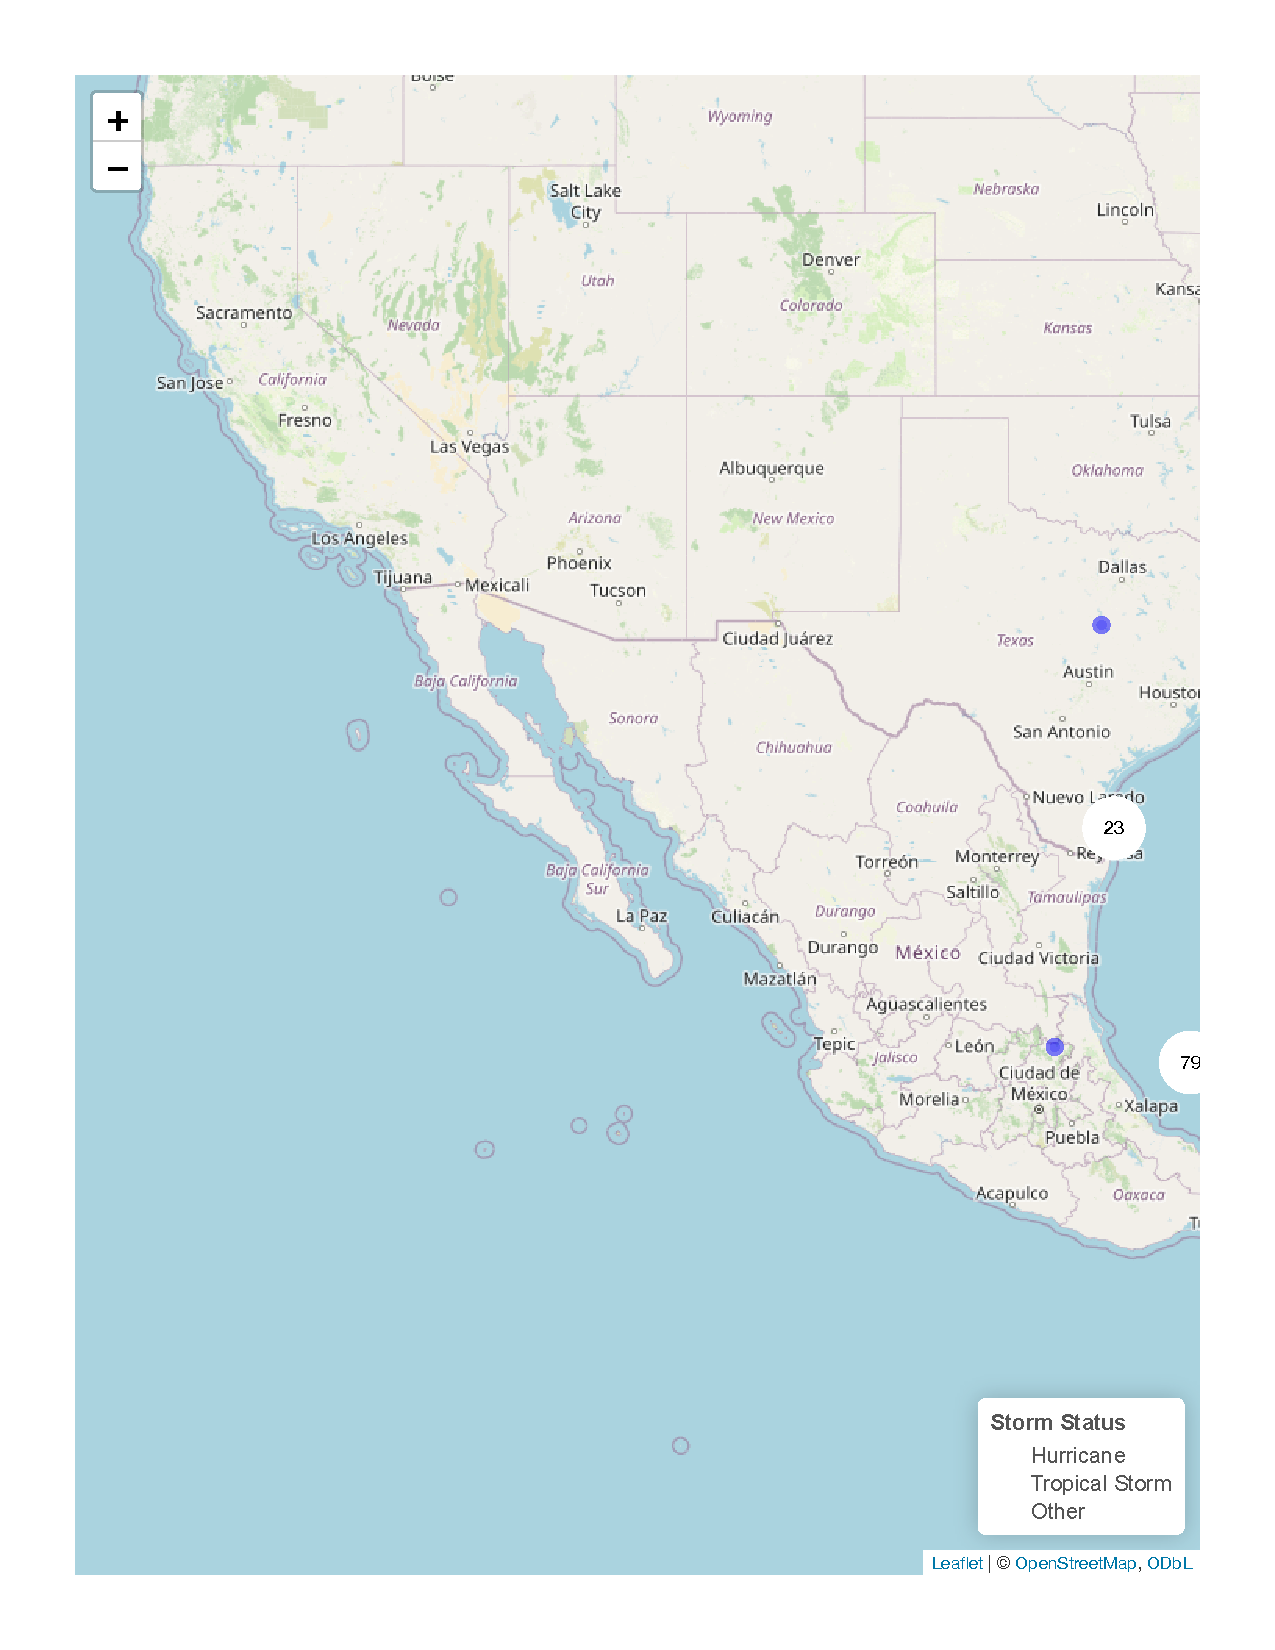
\includegraphics{GroupTask3_files/figure-pdf/LeafletMap-1.pdf}

\subsection{3.4 Statistical Analysis}\label{statistical-analysis}

\begin{Shaded}
\begin{Highlighting}[]
\NormalTok{yearly\_storms }\OtherTok{\textless{}{-}}\NormalTok{ recent\_gulf\_storms }\SpecialCharTok{\%\textgreater{}\%}
  \FunctionTok{group\_by}\NormalTok{(YEAR) }\SpecialCharTok{\%\textgreater{}\%}
  \FunctionTok{summarize}\NormalTok{(}\AttributeTok{storm\_count =} \FunctionTok{n}\NormalTok{())}

\FunctionTok{View}\NormalTok{(yearly\_storms)}

\NormalTok{monthly\_storms }\OtherTok{\textless{}{-}}\NormalTok{ recent\_gulf\_storms }\SpecialCharTok{\%\textgreater{}\%}
  \FunctionTok{mutate}\NormalTok{(}\AttributeTok{MONTH =} \FunctionTok{as.numeric}\NormalTok{(}\FunctionTok{substr}\NormalTok{(DATE, }\DecValTok{5}\NormalTok{, }\DecValTok{6}\NormalTok{))) }\SpecialCharTok{\%\textgreater{}\%}
  \FunctionTok{group\_by}\NormalTok{(MONTH) }\SpecialCharTok{\%\textgreater{}\%}
  \FunctionTok{summarize}\NormalTok{(}\AttributeTok{storm\_count =} \FunctionTok{n}\NormalTok{())}

\FunctionTok{View}\NormalTok{(monthly\_storms)}

\NormalTok{status\_count }\OtherTok{\textless{}{-}}\NormalTok{ recent\_gulf\_storms }\SpecialCharTok{\%\textgreater{}\%}
  \FunctionTok{group\_by}\NormalTok{(STATUS) }\SpecialCharTok{\%\textgreater{}\%}
  \FunctionTok{summarize}\NormalTok{(}\AttributeTok{count =} \FunctionTok{n}\NormalTok{())}

\FunctionTok{View}\NormalTok{(status\_count)}
\end{Highlighting}
\end{Shaded}

\begin{Shaded}
\begin{Highlighting}[]
\FunctionTok{ggplot}\NormalTok{(yearly\_storms, }\FunctionTok{aes}\NormalTok{(}\AttributeTok{x =}\NormalTok{ YEAR, }\AttributeTok{y =}\NormalTok{ storm\_count)) }\SpecialCharTok{+}
  \FunctionTok{geom\_line}\NormalTok{(}\AttributeTok{color =} \StringTok{"blue"}\NormalTok{) }\SpecialCharTok{+}
  \FunctionTok{geom\_point}\NormalTok{() }\SpecialCharTok{+}
  \FunctionTok{labs}\NormalTok{(}\AttributeTok{title =} \StringTok{"year storm count from 99{-}23"}\NormalTok{,}
       \AttributeTok{x =} \StringTok{"Year"}\NormalTok{,}
       \AttributeTok{y =} \StringTok{"\# of Storms"}\NormalTok{)}
\end{Highlighting}
\end{Shaded}

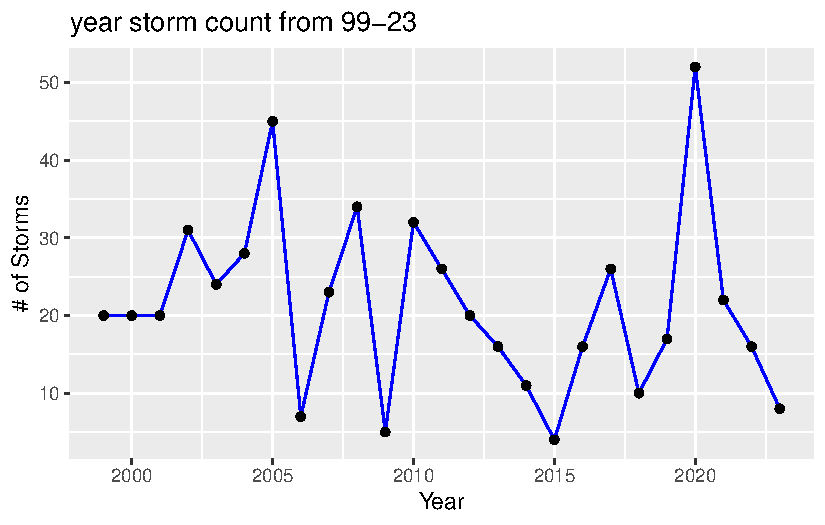
\includegraphics{GroupTask3_files/figure-pdf/Plots-1.pdf}

\begin{Shaded}
\begin{Highlighting}[]
\FunctionTok{ggplot}\NormalTok{(monthly\_storms, }\FunctionTok{aes}\NormalTok{(}\AttributeTok{x =}\NormalTok{ MONTH, }\AttributeTok{y =}\NormalTok{ storm\_count)) }\SpecialCharTok{+}
  \FunctionTok{geom\_col}\NormalTok{(}\AttributeTok{fill =} \StringTok{"steelblue"}\NormalTok{) }\SpecialCharTok{+}
  \FunctionTok{labs}\NormalTok{(}\AttributeTok{title =} \StringTok{"monthly storm freq"}\NormalTok{,}
       \AttributeTok{x =} \StringTok{"Month"}\NormalTok{,}
       \AttributeTok{y =} \StringTok{"\# of Storms"}\NormalTok{) }\SpecialCharTok{+}
  \FunctionTok{scale\_x\_continuous}\NormalTok{(}\AttributeTok{breaks =} \DecValTok{1}\SpecialCharTok{:}\DecValTok{12}\NormalTok{,}
                     \AttributeTok{labels =} \FunctionTok{c}\NormalTok{(}\StringTok{"Jan"}\NormalTok{, }\StringTok{"Feb"}\NormalTok{, }\StringTok{"Mar"}\NormalTok{, }\StringTok{"Apr"}\NormalTok{, }\StringTok{"May"}\NormalTok{, }\StringTok{"Jun"}\NormalTok{, }
                                \StringTok{"Jul"}\NormalTok{, }\StringTok{"Aug"}\NormalTok{, }\StringTok{"Sep"}\NormalTok{, }\StringTok{"Oct"}\NormalTok{, }\StringTok{"Nov"}\NormalTok{, }\StringTok{"Dec"}\NormalTok{))}
\end{Highlighting}
\end{Shaded}

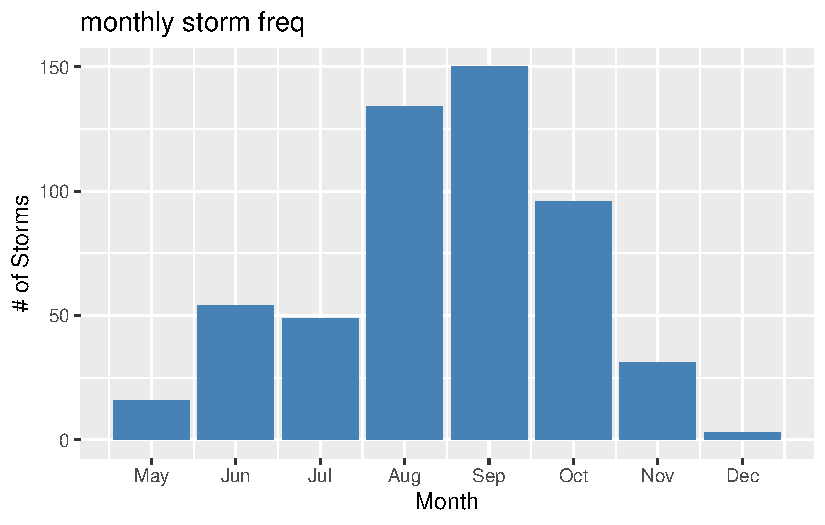
\includegraphics{GroupTask3_files/figure-pdf/Plots-2.pdf}

\begin{Shaded}
\begin{Highlighting}[]
\FunctionTok{ggplot}\NormalTok{(status\_count, }\FunctionTok{aes}\NormalTok{(}\AttributeTok{x =}\NormalTok{ STATUS, }\AttributeTok{y =}\NormalTok{ count, }\AttributeTok{fill =}\NormalTok{ STATUS)) }\SpecialCharTok{+}
  \FunctionTok{geom\_bar}\NormalTok{(}\AttributeTok{stat =} \StringTok{"identity"}\NormalTok{) }\SpecialCharTok{+}
  \FunctionTok{labs}\NormalTok{(}\AttributeTok{title =} \StringTok{"strm count by status"}\NormalTok{,}
       \AttributeTok{x =} \StringTok{"Status"}\NormalTok{,}
       \AttributeTok{y =} \StringTok{"\# of Storms"}\NormalTok{) }\SpecialCharTok{+}
  \FunctionTok{scale\_fill\_manual}\NormalTok{(}\AttributeTok{values =} \FunctionTok{c}\NormalTok{(}\StringTok{"HU"} \OtherTok{=} \StringTok{"red"}\NormalTok{, }\StringTok{"TS"} \OtherTok{=} \StringTok{"orange"}\NormalTok{, }\StringTok{"TD"} \OtherTok{=} \StringTok{"blue"}\NormalTok{))}
\end{Highlighting}
\end{Shaded}

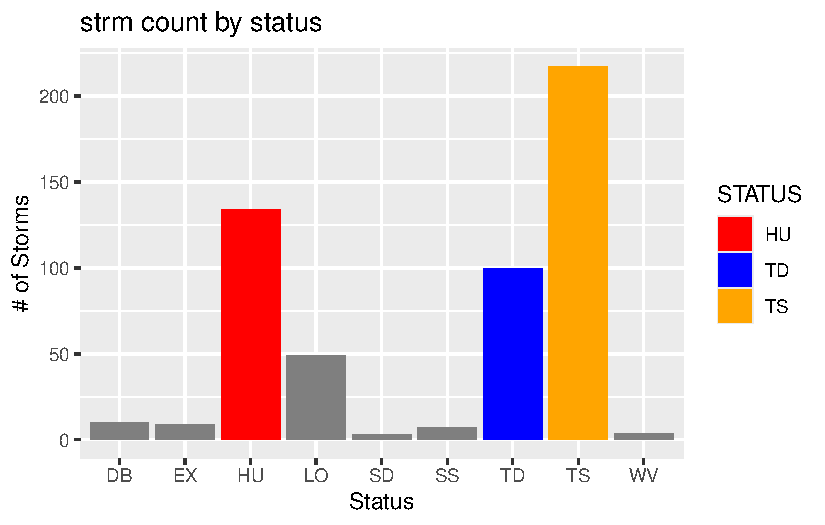
\includegraphics{GroupTask3_files/figure-pdf/Plots-3.pdf}

\begin{Shaded}
\begin{Highlighting}[]
\NormalTok{intensity\_trend }\OtherTok{\textless{}{-}}\NormalTok{ recent\_gulf\_storms }\SpecialCharTok{\%\textgreater{}\%}
  \FunctionTok{group\_by}\NormalTok{(YEAR) }\SpecialCharTok{\%\textgreater{}\%}
  \FunctionTok{summarize}\NormalTok{(}\AttributeTok{avg\_windspeed =} \FunctionTok{mean}\NormalTok{(WINDSPEED\_KT, }\AttributeTok{na.rm =} \ConstantTok{TRUE}\NormalTok{))}

\FunctionTok{ggplot}\NormalTok{(intensity\_trend, }\FunctionTok{aes}\NormalTok{(}\AttributeTok{x =}\NormalTok{ YEAR, }\AttributeTok{y =}\NormalTok{ avg\_windspeed)) }\SpecialCharTok{+}
  \FunctionTok{geom\_line}\NormalTok{(}\AttributeTok{color =} \StringTok{"darkred"}\NormalTok{) }\SpecialCharTok{+}
  \FunctionTok{geom\_point}\NormalTok{() }\SpecialCharTok{+}
  \FunctionTok{labs}\NormalTok{(}\AttributeTok{title =} \StringTok{"Avg Storm Intensity Over Time 99{-}23"}\NormalTok{,}
       \AttributeTok{x =} \StringTok{"Year"}\NormalTok{,}
       \AttributeTok{y =} \StringTok{"Avg Wind Speed (kt)"}\NormalTok{)}
\end{Highlighting}
\end{Shaded}

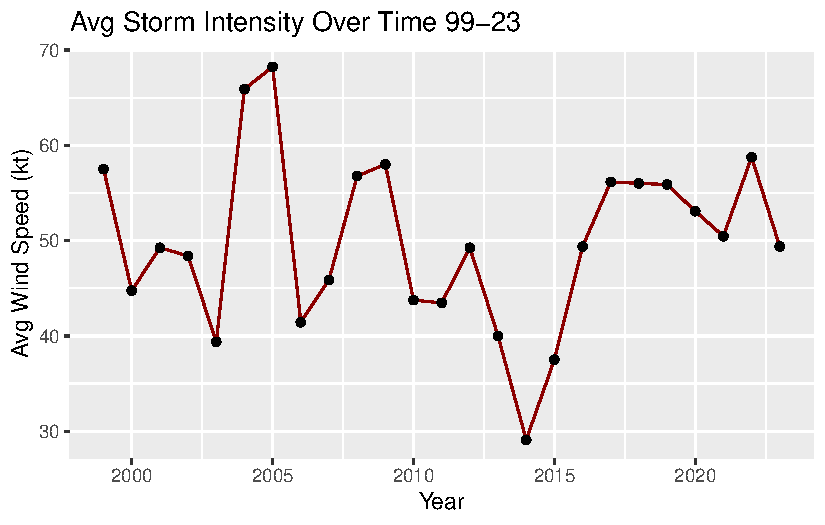
\includegraphics{GroupTask3_files/figure-pdf/Plots-4.pdf}

\newpage

\section{4.0 Results}\label{results}

Here you can discuss the findings from your statistical analysis and
visualizations.

\newpage

\section{5.0 Discussion}\label{discussion}

Discuss the implications of your findings and their significance for
hurricane risk assessment.

\newpage

\section{6.0 Conclusion}\label{conclusion}

Summarize your key findings and their implications for hurricane risk
assessment in the Gulf of Mexico region. \newpage \# References
\{.unnumbered\}

\printbibliography[heading=none]

\printbibliography[heading=bibintoc,title={References}]
\end{document}
